\section{Identity federations}
\subsection{What is an identity federation?}

A simple identity federation example is when signing in to "antagning.se". 
The user visits "antagning.se", needs to visit "my pages", to do so he/she presses "Log in". 
Assuming the user is already studying in Sweden perhaps at Lule\r{a} University of Technology he/she 
can select this university among the listed universities. 
The user has made his/her choice and is redirected to the selected university's student portal and is identified through the university. 

An identity federation can be based on different standards.
The identity federation used in the thesis work testing environment is based on OASIS Security Assertion Markup Language (SAML 2.0) \cite{pdf:oasis-open-core,pdf:oasis-open-metadata,pdf:oasis-open-metadata-profile,pdf:oasis-open-bindings,pdf:oasis-open-profiles,pdf:oasis-open-glossary,pdf:oasis-open}. 
The SAML technical overvew \cite[p.~8]{pdf:oasis-open} describes SAML as an XML-based framework both for
describing and exchanging security information between business partners online.    

\begin{figure}[ht]
\begin{center}
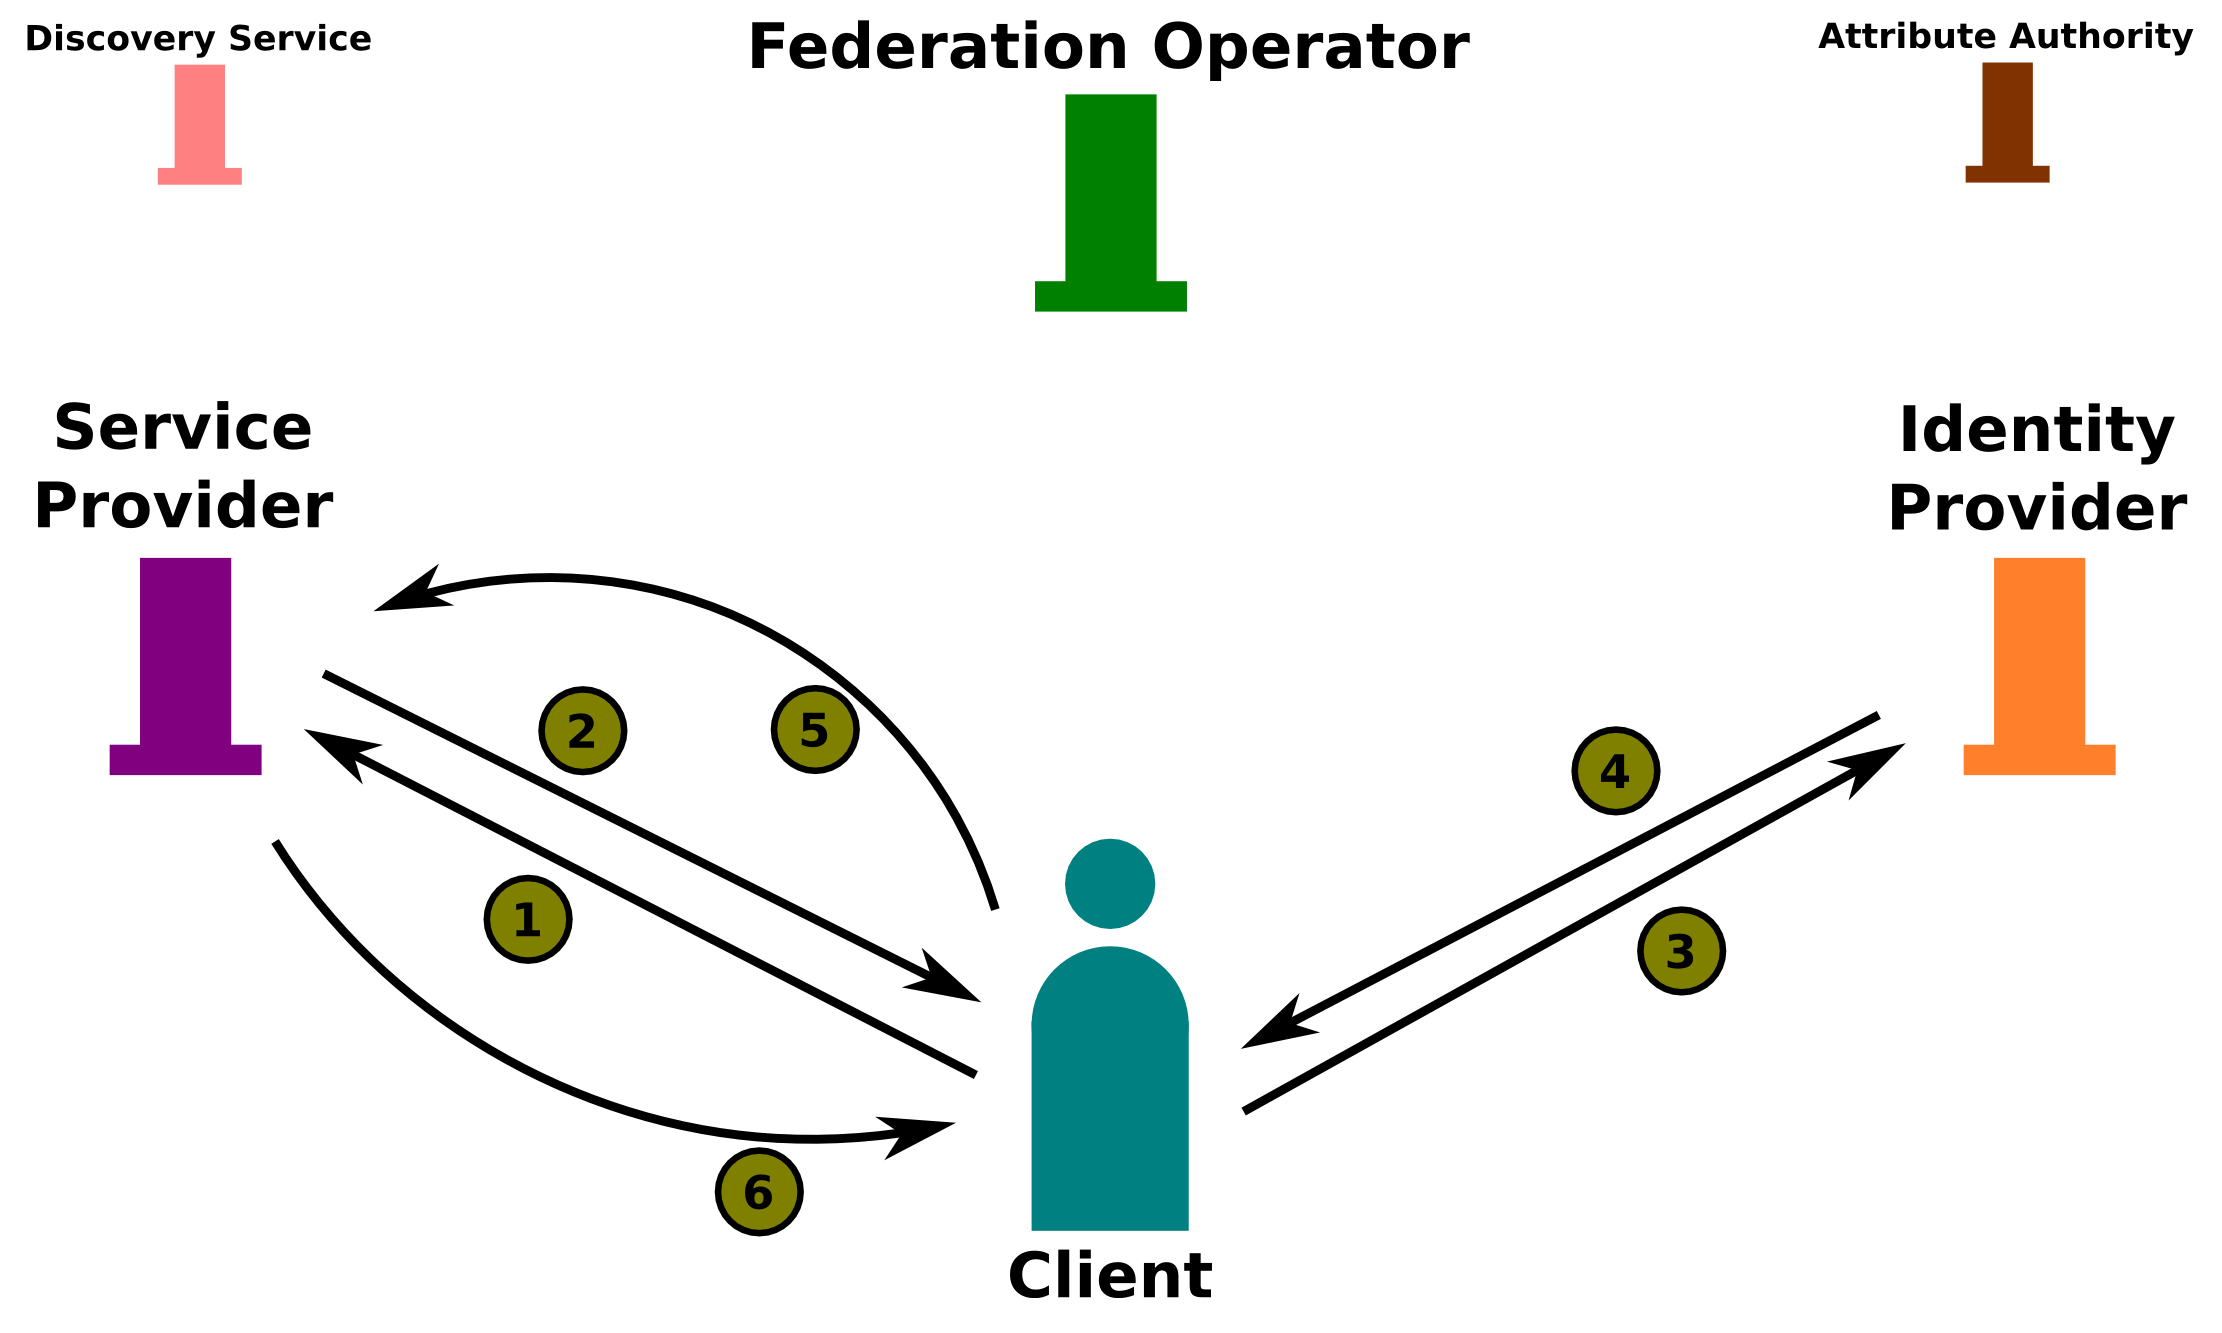
\includegraphics[scale=1]{Figures/identityFed.png}
\end{center}
\caption{Shows how the client visits the service provider (1). 
The client want to see restricted resources at the service provider, whom demands that the client is identified first. 
Therefore, the service provider redirects the client to the identity provider (2) and (3). 
At the identity provider, the client is authenticated and sent back to the service provider (4) and (5). 
The client is now allowed to see restricted resources at the service provider (6).\label{ch3:IdentityFed}}
\end{figure}


In SAML standard "antagning.se" is a service provider (SP) \cite[p.~11]{pdf:oasis-open-glossary} and the identification at 
Lule\r{a} University of Technology is the identity provider (IdP) \cite[p.~7]{pdf:oasis-open-glossary}, see figure \ref{ch3:IdentityFed}.
The discovery service (Disco) is where the user could chose from several universities at "antagning.se".
Furthermore, SAML also specifies the Attribute Authority (AA) that provides 
a "ticket" containing information about the user from a third party perspective. A theoretical AA example is "Skatteverket", it wants to 
allow an individual to see their tax account, both the business as well the people it involves. 
"Skatteverket" sends an attribute request to "Bolagsverket" that will answer this request 
with a "ticket" containing information that allows or disallows the individual to see his/her tax account \cite[p.~284]{pdf:SOU}.

Outside the SAML standard, the identity federation can also have a federation operator. It is possible to have an identity federation both 
with and without a federation operator. 
The federation operator provides digitally signed aggregated metadata \cite[p.~3]{pdf:Skolfederation}. 
"Metadata defines a way to express and share configuration information between SAML parties.
For instance, an entity's supported SAML bindings, operational roles (IDP, SP, etc), identifier information,
supporting identity attributes, and key information for encryption and signing can be expressed using SAML
metadata XML documents. SAML Metadata is defined by its own XML schema" \cite[p.~16]{pdf:oasis-open}.
The key information refers to the shared certificates (public keys) that are used when connecting and sending requests and responses 
messages between the entities.
With that said every service provider and identity provider holds the shared certificates between each other within its metadata. 

The need of a federation operator grows as the amount of service- and identity providers grows,
since it provides that every service- and identity provider can turn to the federation operatior to make sure the metadata is up to date 
instead of having to turn to each other. 
The only thing is that the service- and identity providers has to keep track of a shared certificate with the federation operator, 
meanwhile, the federation operator provides them with a metadata file containing every ones certificates.
A federation operator also provides a unity between the entities in the federation. This unity can be used so that every entity share 
administration, has the same technical set up and so on.

\subsection{The technical side of an identity federation}
The example above with "antagning.se" is in SAML referred to as a SP-initiated web SSO  \cite[p.~12]{pdf:oasis-open}, 
where SSO stands for Single Sign-On. SSO is when it is possible to sign in at one place and use that identification at other places as well. 

SP-initiated web SSO uses The Web Browser SSO Profile that says that "to implement this scenario,
a profile of the SAML Authentication Request protocol is used, in conjunction with the HTTP Redirect, HTTP POST and
HTTP Artifact bindings" \cite[p.~14]{pdf:oasis-open-profiles}.

In more technical terms the SP-initiated web SSO scenario, see figure \ref{ch3:IdentityFed} 
is in the SAML Profiles document \cite[p.~15]{pdf:oasis-open-profiles} described 
as the client (principal) sends an HTTP request via an HTTP user agent asking to access a protected 
resource at the SP. The client is not authenticated and therefore the SP
obtains with the authentication request protocol the location to the IdP. The SP then issues an "AuthnRequest" message
that the user agent deliver to the IdP through an HTTP redirect, post or artifact binding.
At the IdP the client is identified through some back-end engine with user credentials, in
our testing environment Lightweight Directory Access Protocol (LDAP) is used more specifically OpenLDAP \cite{website:openldap}.
The IdP then issues a "Response" message that the user agent deliver to the SP through HTTP post or artifact binding.
This message holds at least one authentication assertion as well as attributes that describes the user or it may hold an error.
Depending on the respons message the client will receive access to the SP or not.
\section{Certificates}
\subsection{Certificates in general}

This section describes how certificates is used to send a private message from Alice to Bob, the technical steps from encryption 
of the message to the validation of trust.
The example is based on the introduction on SSL/TLS from the Apache Foundation \cite{website:ssl_intro}.
%Alice and Bob with the help of a signed certificates and is based on\cite{website:ssl_intro}. 

Public key cryptography algorithm transforms a message from Alice in to a private (encrypted) message to Bob, 
the message is unreadable until it is decrypted. 
Encrypted messages can only be decrypted with a secret key, in public key cryptography two keys are used that both can encrypt and 
decrypt messages. 
However if one key is used to encrypt the message only the other key can decrypt it, which make publication of the public key 
possible while keeping the private key secret. 
Additionally, if Alice and Bob has shared keys, Alice can encrypt the private message with the public key and only Bob 
with the private key can decrypt the message.

The possibility that someone has made changes to the message still exist since the public key is public. 
"Message digest" even called one-way function or hash function can be used to guarantee that the message has not changed. 
Message digest creates a short, fixed-length representation of the message about to be sent and sends the message and
the summary to Bob.
Then Bob when receives the message he makes a summary as well and compares it with Alice's.

In addition, the message digest has to be securely sent as well, which is made possible with digital signatures. A digital signature
is made by the private key by encrypting a digest of the message and other information as well, sequence number for example.
It is Alice that creates the digital signature and includes it in the message digest to Bob and since no one can change the digest and still 
sign it, the integrity is kept. Moreover, to make sure reuse of the signature can not be made at a later date, the signature contains a 
sequence number that is unique. 

Furthermore, Alice needs to know that the shared public key is with Bob as well as Bob needs to verify that the message signature 
really was signed by Alice's private key. With a certificate that validates the other's identity, confirms the public key and
is signed by a Certificate Authority (CA), Alice can be sure she is talking to Bob and vice versa.

\subsubsection{Certificates and security}
Certificates are not secure in themselves the security is built on cryptographic algorithms and most often on public-key cryptography also called asymmetric cryptography.
Cryptography is about analysing and breaking ciphers, it provides secure communication between the message sender and receiver. 
Cryptographic algorithms uses keys to protect data, in public-key cryptography a public encryption key and a private (secret) decryption key is used. \cite[p.~252]{book:computer-security}

The RSA algorithm has become almost synonymous with public key cryptography according to Computer Networking, A top down approach \cite[p.~726]{book:computer-networking}.
This book also informs that RSA uses arithmetic modulo-n operations as well as it describes how the recipient generates his/her private and public RSA key.
RSA is secure since there are no known algorithms that quickly can factor large prime numbers and the larger the generated prime numbers are, the more secure the keys become.

\subsection{Certificates in SAML}

Saml2int \cite{website:saml2int} describes an Interoperable SAML V2.0 Web Browser SSO Deployment Profile that is based on 
SAML Web Browser SSO Profile in the SAML Profiles document\cite{pdf:oasis-open-profiles}. 
The deployment profile describes the behaviour and options that all parties are supposed to follow. 
Furthermore, it addresses the content, exchange and processing of SAML messages.
For example in the Saml2int profile \cite{website:saml2int}, the service provider should at endpoint protect response 
messages using Transport Secure Layer (TLS) or Secure Sockets Layer (SSL)  and identity providers should do the same when receiving 
authentication request. 
However, if an identity provider does not use TLS/SSL, XML Encryption should be used and in its response message return an encrypted assertion. 
In addition, if service providers does not use TLS/SSL as recommended, then the service providers metadata should include a suitable key descriptor for XML Encryption.

%A TLS/SSL handshake example adapted to the identity federation influenced by \cite{website:ssl_explained}.
%The client initiates the handshake by connecting to the service provider with TLS/SSL on port 443. 
%Continues with sending basic information to the service provider, whom respond with sending basic 
%information as well as its certificate and public key back. 
%The client validates the certificate and public key with the CA as mentioned in certificates in general above. 
%Additionally, if the validation was successful the client generates a secret key to be used during the session and 
%sends the key encrypted to the service provider completing the handshake. 

\section{DNS-Based Authentication of Named Entities} 
\subsection{In general}
DANE, DNS-based Authentication of Named Entities, is as of writing still a new concept and technology.
It's introduced with the informational RFC document\cite{rfc:6394} describing some use cases and one use case specified in more detail in the Internet-Draft "The DNS-Based Authentication of Named Entities (DANE) Protocol for Transport Layer Security (TLS)"\cite{rfc:draft-dane}.
After the specfication for TLS communication, S/MIME is up next, which will describe how to map an emailaddress to a resource record.
Exactly how this will work and which resource record type that must be used is not yet clear according the to the draft\cite{rfc:draft-smime}.
Make note that these Internet-Drafts from the Internet Engineering Task Force (IETF) is still "work in progress" as they are still drafts and may change.

The problem that DANE tries to solve is the current issue with Certificate Authorities (CAs) where anyone of them may give out a certificate for any domain name.
It might not be likely that a CA loses its private key but might sign a certificate with information that is not correct or the CA might sign a key that is intended for signing/encrypting emails but is than used in other settings.
%It might not be likely that a CA signs a certificate that doesn't come from the true owner of a domain name though the CA might be hacked and lose their private key or the CA might sign a key that should be used for signing emails but is then used for something else.

A hacker that gets hold of the private key of a CA would get the ability to create a new signed certificate for any domain of his/her choice.
As the model with CAs works today where they can sign any domain name and the more common webbrowsers (Mozilla Firefox, Microsoft Internet Explorer, Google Chrome) trust most of these CAs, the new signed certificate from the hacker will give clients connecting to the server with the false certificate a "false-positive".
The domain name matches the common name in the certificate and it's signed by one of all trusted/well-known CAs.
This is where DANE comes in as a solution.

\begin{figure}[ht]
\begin{center}
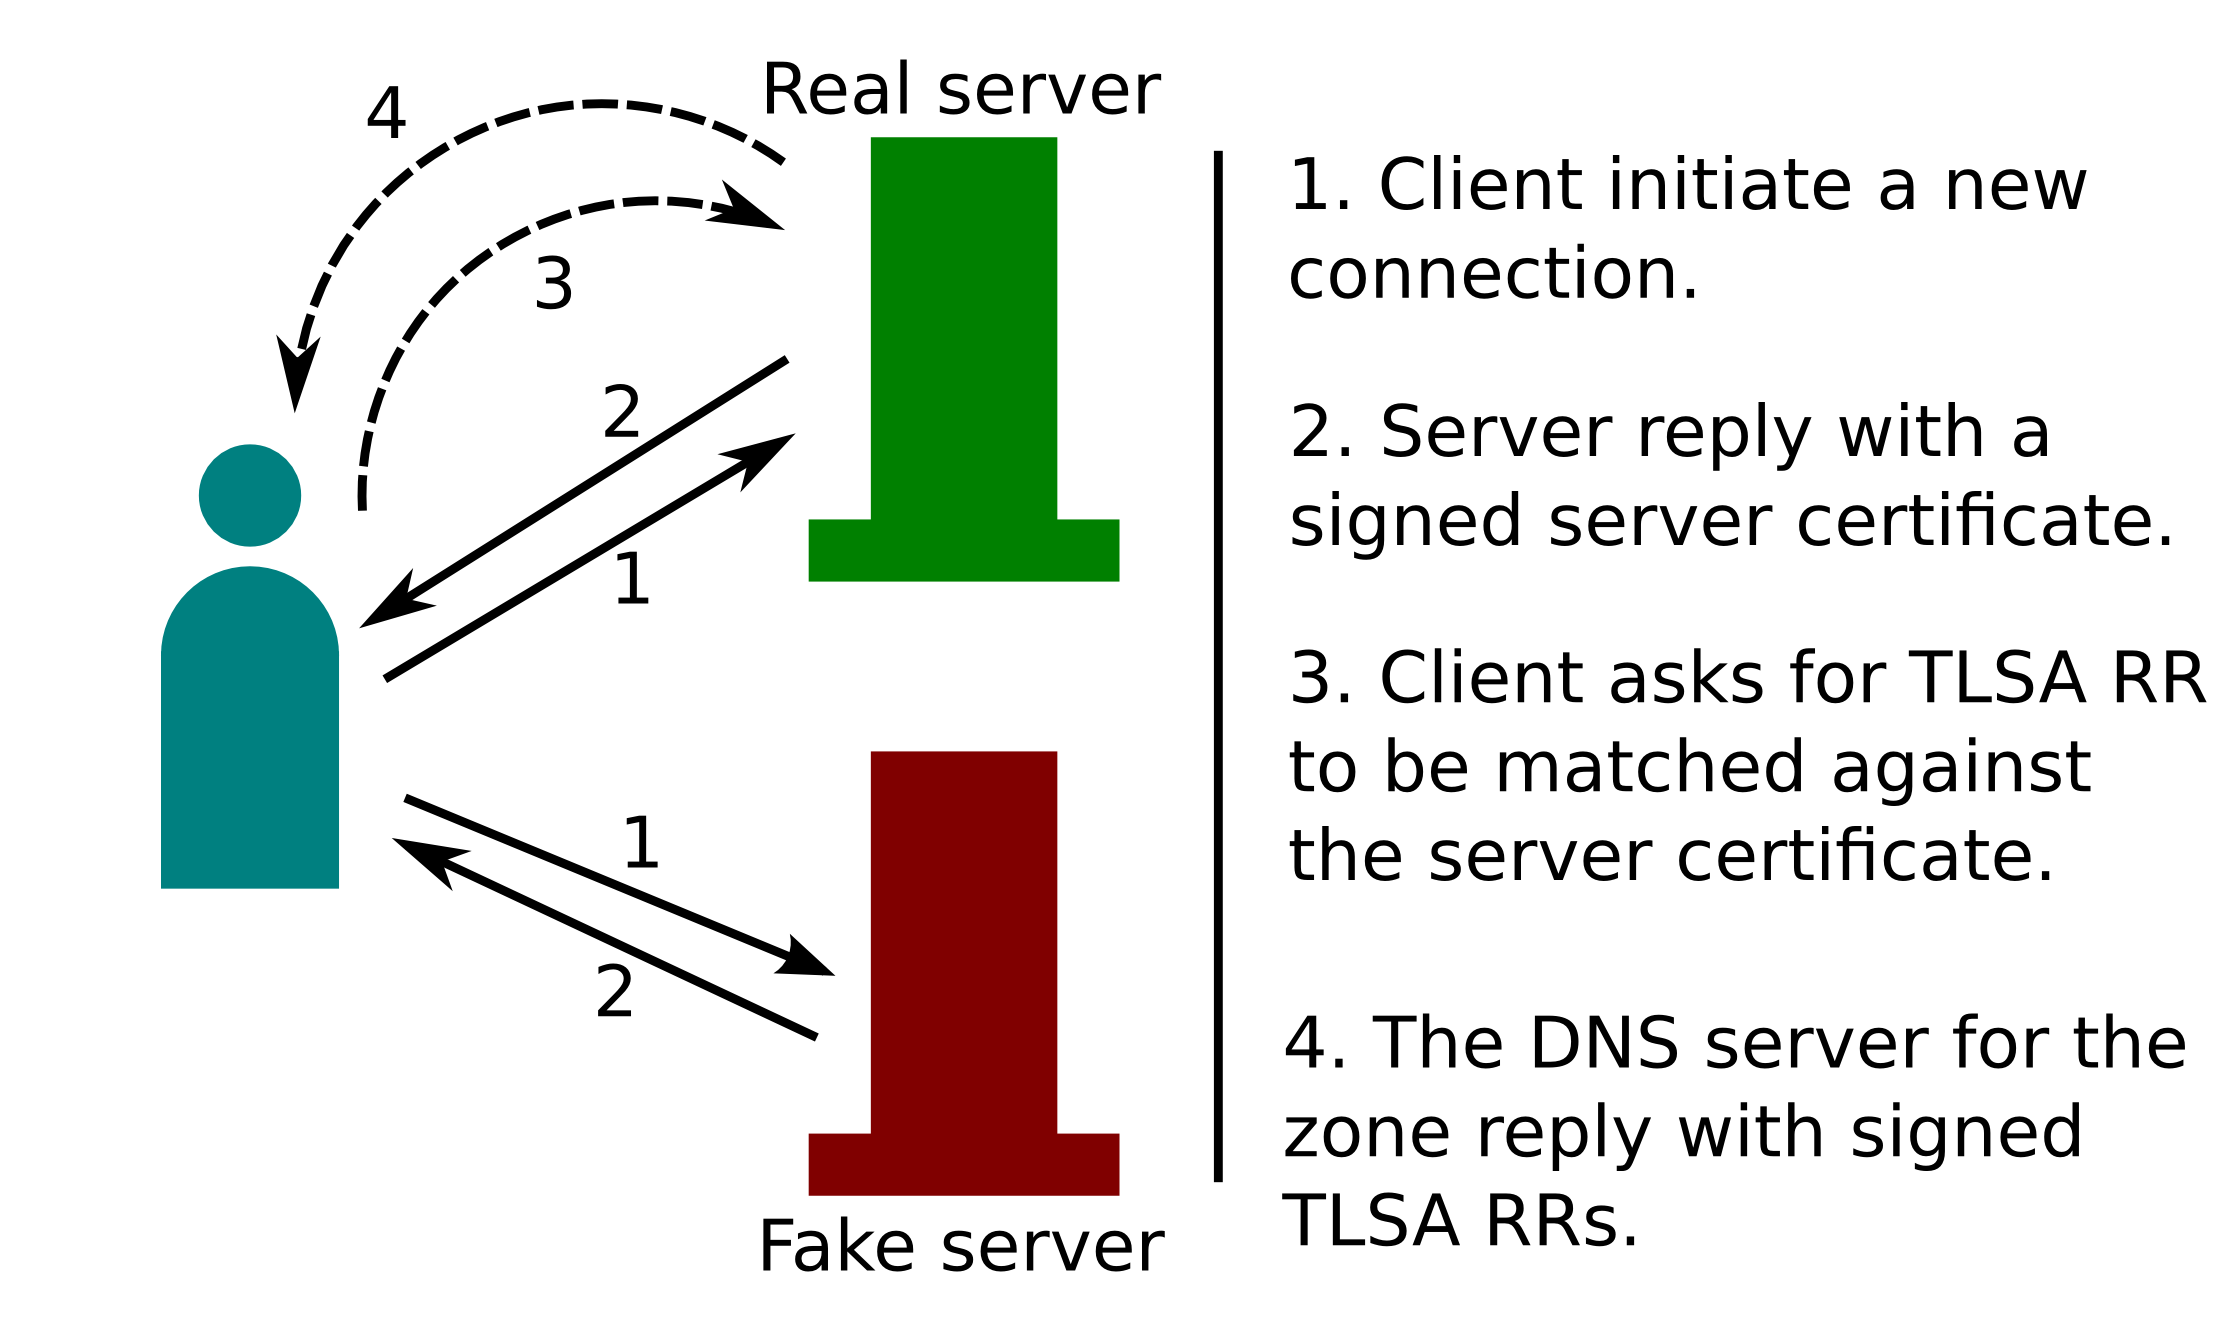
\includegraphics[scale=1]{Figures/daneWithTlsa.png}
\end{center}
\caption{A client connect to either a real or fake server. The third and fourth step is done within the Domain Name System and requires DNSSEC active. (It is assumed that both the real and the fake server has a server certificate signed by some well-known CA for the same domain.)\label{ch3:daneWithTlsa}}
\end{figure}

The following explanation is also presented in figure \ref{ch3:daneWithTlsa}.
If the client connecting to the false server could get some information about which certificate is the true one to use, the client would know that the false certificate is a false one and not to trust it.
In short, this works by trusting the DNSSEC infrastructure and the owner of a domain name can publish a TLSA DNS resource record (for TLS communication) which tells the client which certificate is the correct one to use.
If the hacker tried the same attack with DANE fully operational he/she would not succeed cause the client would know that the false certificate from the hacker (fake server) is actually a false one.
%This is what happens in figure \ref{ch3:daneWithTlsa} when the client can compare the server certificate (recieved in step 2) with the TLSA resource record (recieved in step 4).
The client would in this case immidiately drop all established connections, if any, and never initiate a new TLS connection.

This effectively moves some responsiblity from the CAs to the domain owner.
The domain owner now has full control of which TLS certificates are the valid ones.

\subsection{An example}
How DANE works in detail for TLS communication is specified in the Internet-Draft earlier mentioned\cite{rfc:draft-dane} but to be able to follow later reasoning a short presentation will be given here.
Let's take an example, Alice wants to get hold of some resource from Bob that needs to be protected so only Alice and Bob knows about it and noone tampers with it while in transit.
This is where TLS comes into play.
Alice initiate a TLS handshake as a TLS client with Bob which in this example is acting as TLS server. 
Everything works fine and with TLS they setup a secure channel between themselves.

\begin{figure}[ht]
\begin{center}
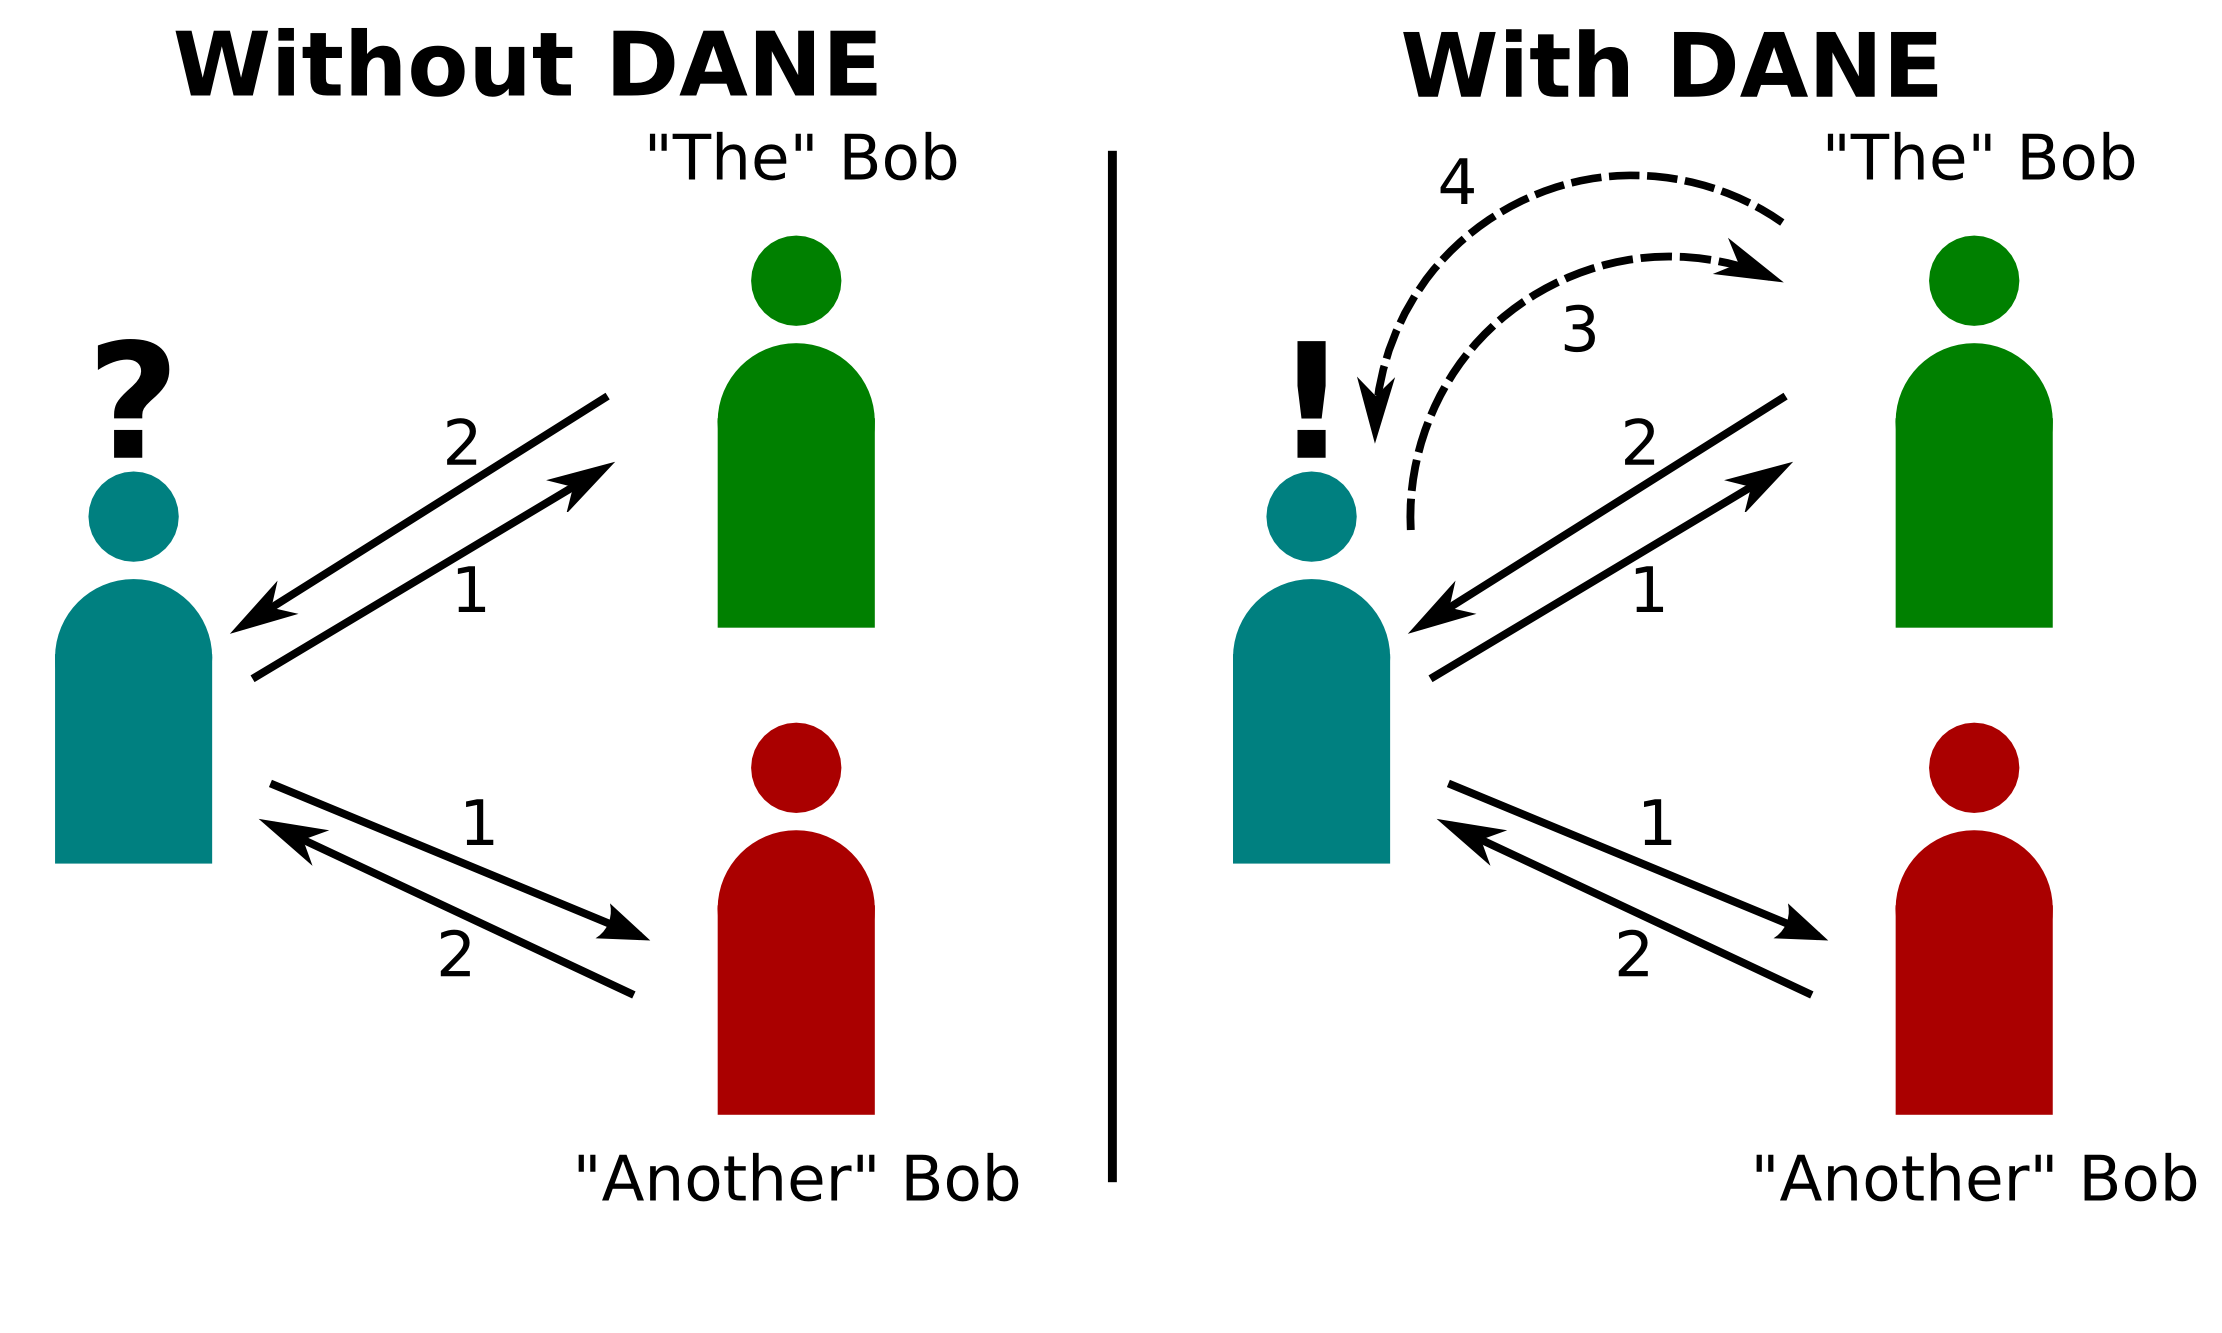
\includegraphics[scale=1]{Figures/daneWithAndWithoutDane.png}
\end{center}
\caption{Without DANE the connecting client can't be sure without some out-of-band procedure or prior communication who is the real Bob. With DANE "the" Bob can publish a TLSA RR which will determine which TLS server certificate is the real one. (This assumes that both the client and "the" Bob trust the DNSSEC infrastructure).\label{ch3:daneWithAndWithoutDane}}
\end{figure}


But hold on, how does Alice know that she is communicating with "the" Bob she believes it is or is it someone else that is trying to fake the identity of "the" Bob?
To perhaps give a better explanation figure \ref{ch3:daneWithAndWithoutDane} describe this dilemma.

In the initial TLS handshake Alice retrieves a server certificate that she needs to validate with a third party, a CA.
This is a certificate from Bob that is signed by his CA of choice, which basically says that the CA in question has confirmed, in some out-of-band way, that it's the true Bob, Alice is communicating with.

In this scenario, similiar to the scenario with the "hacker" above, there is no way for Bob as server/domain owner to limit which certificates that is allowed to be used for his domain.
A hacker with a certificate for Bob's domain signed by any well-known CA will be able to set up his/her valid TLS server in the name of Bob.
Alice will then never know if it really is "the" Bob she is communicating with next time.

To prevent this Bob can publish TLSA DNS resource records (TLSA RRs)\cite[ch. 2]{rfc:draft-dane} with either the full certificate or a hash value of it.
Alice can when initiating the TLS handshake also ask for the TLSA RRs from Bob.
With DNSSEC in place she can be sure that she recieves the TLSA RR from the true Bob and if the resource records matches the given certificate that was given in the TLS handshake Alice is sure it's to "the" Bob she is opening a secure channel.

Depending on the TLSA RR information and local policies Alice might have to do the the normal certificate chaining to some trusted anchor aswell or she will accept a self-signed certificate from Bob.
TLSA resource records is a new DNS record type that is still not approved as a standard so it might change in the future before being approved.

% TODO: Give more in depth presentation about certificate here?
% TODO: Mention anywhere what root certificates are and how they're used?
% TODO: What is well-known CAs?

% Removed by Christoffer, 2012-04-19: As the Internet-Draft specifies the first octet in the TLSA RR is allocated for "certificate usage", the parts concerning TLS only allocates five out of these 256 possible values so future standards can use the same resource record type and only allocating one of the free "certificate usage" fields.
% Removed by Christoffer, 2012-04-19: This means that if a new standard is created that doesn't make use of TLS but needs certificate in some other way it might make sense to allocate a "certificate usage" number within the TLS RR instead of creating whole new resource record type.

% TODO: ADD: With DANE the CA system remains the same with two big differences.
% (1) Without DANE all CAs are as weak as the weakest CA. Every CA needs to make sure to keep their private keys/certificate safe.
% If anyone of them brakes, all CAs lose trust. With DANE only domains originally signed by themselves is in danger for false certificate so if a warning goes out fast when the break-in is noticed...zone administrators in danger can revoke their certificates asap and publish a new in the DNS system. (Though even the false certificate from the hackers may not be of any help)...though better be safe than sorry if any private key from a CA is lost.
% (2) With DANE it will still be possible to hack a CA and create false certificate for any domain but with DANE the additional check can be made through the DNS system and the zone owner/administrator has the last say when it comes to which certificates that are the true ones.

\section{How DANE can be implemented in Shibboleth}
Shibboleth is not a single computer program, it's more of a software package consisting of an identity provider written in java and a service provider written in C++ as the main parts in the package.
As dependency for the identity provider and service provider software, Opensaml exist both in Java and C++.
Other projects are a centralized discovery service, embedded discovery service and  metadata aggregator among others.
Even if Shibboleth can be viewed as a software package, all parts can and usually are installed seperately on different machines.

DNS-Based Authentication of Named Entities (DANE) is still a draft for TLS and S/MIME communication and the RFC available is only an informational RFC focusing mainly on TLS use cases.
The main concept is that with DNSSEC in place it's possible to use the DNS system as a trusted source for retrieval of some extra information that confirms what earlier was made in some other out-of-band way.
As an example it's possible to trust a TLS certificate retrieved when establishing that connection because it's possible to retrieve extra information through the DNS system that proves it's the right certificate in use.

Focus in this project has been on the identity provider part in Shibboleth.
It has good documentation on how to extend it. 
Make note that the identity provider software is currently at version 2.3.6 and a new major version is on the way as 3.0.0.
The identity provider software has both an API and different extension points.


%Migh be implemented as a filter in shibboleth IdP
%There are several "layers" in the Shibboleth software
%Shibboleth uses OpenSAML and OpenSAML uses OpenSSL(confirm this later on.)

%DNS (Domain Name System) is the Internets domain name system, a hierarchic and distributed database that makes it possible to quickly find information about which IP-address (and other information) that is connected to a domain name. \cite[p.~64]{book:guide_dns}

%DNSSEC (Domain Name Security Extensions) is a securitylayer added to DNS to secure system against assults like cachingpoisning through signing DNS-data digitaly.\cite[p.~64]{book:guide_dns}

%\section{Theories}

%How do they work together?

%\section{Tools}

%Software? Shibboleth?


%THEORY 
%Background, 
%theories, 
%tools, 
%and anything else that can be used in your work.
%These are largely determined by your purpose and delimitations. This puts your investigation
%in its scientific context.
